\documentclass[11pt,a4paper]{article}
\usepackage[margin=2.5cm]{geometry}
\usepackage[T1]{fontenc}
\usepackage[utf8]{inputenc}
\usepackage[spanish,es-tabla]{babel}
\usepackage{lmodern,microtype,booktabs,graphicx,xcolor,hyperref,amsmath,amssymb,float,enumitem}
\hypersetup{colorlinks=true,linkcolor=blue!50!black,citecolor=blue!50!black,urlcolor=blue!50!black}
\graphicspath{{report_assets/}}
\newcommand{\acc}{\mathrm{acc}}
\setlength{\emergencystretch}{4em}

\title{CS-NAS: búsqueda evolutiva de arquitecturas federada con muestreo estratificado por clusters de similitud\\[2pt]\large Informe experimental final (resultado mayormente negativo)}
\author{Proyecto EvoFederated}
\date{21 de octubre de 2026}

\begin{document}
\maketitle

\begin{abstract}
\noindent Se propuso y evaluó CS-NAS, un algoritmo evolutivo de búsqueda de arquitecturas en aprendizaje federado non-IID con muchos nodos. Los nodos se agrupan una sola vez por similitud de las actualizaciones de un modelo sonda; en cada generación se elige un representante al azar por cluster, esos representantes entrenan cada arquitectura candidata con FedAvg y otro miembro del mismo cluster, que no entrenó, la evalúa. El fitness es la accuracy estimada y el número de parámetros. Se midió: (i) la calidad del estimador de fitness, (ii) la calidad de los frentes de Pareto encontrados frente a muestrear nodos al azar y frente a búsqueda aleatoria, (iii) el ruido del fitness y (iv) un refinamiento multifidelidad. \textbf{Resultados.} Evaluar en un nodo retenido del cluster elimina un sesgo optimista y reduce el RMSE del estimador entre 21\,\% y 48\,\% según régimen y muestreo (41--48\,\% con clusters por $\Delta$). Los clusters por $\Delta$ aproximan a los formados con las etiquetas reales sin usarlas y tienen menor error de evaluación que muestrear nodos al azar, pero no ordenan mejor las arquitecturas (Kendall $\tau$ entre 0.82 y 0.97 en todas las variantes y regímenes, sin diferencias claras entre ellas). En la búsqueda (Fashion-MNIST, $\alpha=0.1$, $N=100$, $C=10$, 5 semillas pareadas, igual coste) CS-NAS no mejora el frente: es ligeramente peor que NSGA-II con nodos aleatorios (diferencia de hipervolumen en test $-0.009$, intervalo $[-0.012,-0.005]$, 0 de 5 semillas a favor) y no se distingue de la búsqueda aleatoria con los mismos clusters. Un control añadido (búsqueda aleatoria con nodos aleatorios) muestra que, con muestreo aleatorio de nodos, NSGA-II supera a la búsqueda aleatoria en el área bajo la curva de hipervolumen en 5 de 5 semillas ($+0.023$, $[+0.016,+0.029]$) y por poco en el hipervolumen final de test ($+0.008$, $[-0.001,+0.019]$, 4/5), un efecto pequeño que no aparece con clusters. El diseño solo detectaría efectos mayores que $\approx$5.7\,\% del hipervolumen en el contraste con clusters. El cuello de botella es el ruido del fitness: una misma arquitectura cambia $\pm0.06$--$0.10$ de accuracy según qué 10 nodos la entrenan, comparable a la banda que separa a las mejores. Subir $C$ a 20 reduce ese ruido a menos de la mitad, y reevaluar candidatos con más nodos mejora el hipervolumen final como máximo en $\approx$1\,\%. Se concluye que, en el régimen probado, la estratificación por similitud no aporta a la búsqueda, y que la evolución aporta a lo sumo una mejora pequeña y solo con muestreo aleatorio de nodos. El aporte es el diagnóstico y las piezas reutilizables (evaluador retenido, estimador, análisis de ruido), no un método ganador.
\end{abstract}

\section{Contexto y objetivo}
Entrenar y evaluar muchas arquitecturas candidatas en aprendizaje federado es caro, y el coste crece con el número de nodos participantes. La revisión sistemática previa de este proyecto (\texttt{manuscript/main.pdf}) y la lectura de texto completo de los estudios más cercanos mostraron que los trabajos de NAS federado que evalúan candidatos con un subconjunto de clientes lo hacen eligiéndolo al azar \cite{zhu2021realtime} o formando grupos que igualan la distribución de etiquetas global \cite{yuan2022resourceaware}, lo que requiere que los clientes revelen información sobre sus datos; la selección de participantes por similitud o agrupamiento se evalúa sobre todo para acelerar el entrenamiento de un único modelo \cite{bhope2023flips}. Khodak et al.\ señalan además que la validación obtenida de pocos clientes es una señal ruidosa \cite{khodak2021federated}. Con ese contexto se propuso CS-NAS, cuyo objetivo es encontrar un frente de Pareto (accuracy frente a número de parámetros) con un coste de evaluación independiente del número de nodos.

\textbf{Pregunta de investigación.} A igual coste de entrenamiento, ¿el muestreo estratificado por clusters de similitud de actualizaciones produce mejores frentes que muestrear nodos al azar, y la búsqueda evolutiva aporta algo sobre muestrear arquitecturas al azar?

Este informe sustituye a las propuestas anteriores del proyecto (disimilitud/similitud con 8 nodos, many-objective), archivadas en la etiqueta de git \texttt{legacy-final}, cuyos resultados no mostraban ventaja de ninguna estrategia y cuya comparación estaba confundida (con una ronda, las estrategias de pares usaban solo dos subconjuntos distintos de clientes en 56 evaluaciones).

\section{Método: CS-NAS}
\begin{enumerate}[leftmargin=*,itemsep=2pt]
\item \textbf{Sonda (una vez).} Los $N$ nodos entrenan el mismo modelo sonda desde la misma inicialización; solo se envía el vector $\Delta_i$ de cada actualización.
\item \textbf{Clusters.} $k$-means esférico sobre los $\Delta_i$ normalizados da $C$ clusters $G_1,\dots,G_C$.
\item \textbf{Representantes por generación.} Se sortea un nodo $r_c\in G_c$ por cluster con un RNG derivado de la semilla y la generación; los mismos representantes se usan para toda la población de esa generación.
\item \textbf{Entrenamiento y evaluación.} Cada arquitectura se entrena con FedAvg sobre $\{r_c\}$, ponderado por $|G_c|$. Se evalúa en otro nodo $e_c\in G_c\setminus\{r_c\}$ que no entrenó (solo inferencia): $\hat a=\sum_c \frac{|G_c|}{N}\,\acc(e_c)$.
\item \textbf{Fitness (minimización).} $\bigl(-\hat a,\;p/p_{\max}\bigr)$, con $p$ el número de parámetros y $p_{\max}$ el de la arquitectura mayor del espacio.
\item \textbf{Búsqueda.} NSGA-II \cite{deb2002nsga2} que reevalúa padres e hijos con los mismos representantes en cada generación (de lo contrario, fitness medidos con nodos distintos sesgarían la selección). La búsqueda aleatoria recibe el mismo número de evaluaciones por generación.
\end{enumerate}
\textbf{Monitoreo (solo reporte).} El mismo modelo se evalúa en todos los nodos; ese valor nunca entra al fitness ni a la selección (verificado con pruebas unitarias). El coste de búsqueda se mide en entrenamientos locales; el de la sonda ($N$ entrenamientos de una época) se reporta aparte.

\textbf{Decisión de diseño documentada.} Evaluar en el propio representante daba un sesgo optimista de +0.025 a +0.045 en un piloto (el modelo acaba de entrenar con esos datos); por eso se adoptó el evaluador retenido.

\section{Protocolo experimental}
\textbf{Datos.} Fashion-MNIST y CIFAR-10 particionados con Dirichlet ($\alpha\in\{0.1,0.5\}$) entre $N=100$ nodos; cada nodo reserva el 30\,\% de su partición para validación; el conjunto de prueba oficial se reparte aparte entre los nodos y solo se lee en la reevaluación final. \textbf{Entrenamiento.} FedAvg, Adam, tamaño de lote 32, y la configuración elegida en el diagnóstico de la sección~\ref{sec:diag} (lr $10^{-2}$, 2 épocas locales, 20 rondas). \textbf{Espacio.} CNN pequeñas: 1--3 bloques convolucionales (8--64 canales, núcleo 3 o 5, ReLU o ELU, BatchNorm, dropout) y pooling global. \textbf{Métricas.} RMSE, sesgo y Kendall $\tau$ del estimador frente a la accuracy del mismo modelo en todos los nodos; hipervolumen (HV) del frente con punto de referencia fijo $(-\acc=0,\;p/p_{\max}=1.05)$; el HV principal se mide sobre el frente final reentrenado desde cero con los 100 nodos y evaluado en test. \textbf{Réplicas.} 5 semillas de partición pareadas entre métodos (3 en un estudio previo); la unidad de réplica es la semilla. Los intervalos son bootstrap sobre esas semillas y deben leerse como descriptivos: con $n=5$ el test de Wilcoxon no puede dar $p<0.0625$.

\section{Resultados}
\subsection{El régimen de entrenamiento condicionaba todo}\label{sec:diag}
Con Adam $10^{-3}$, 2 épocas y 5 rondas (régimen de los primeros estudios) la accuracy media era de apenas 0.18 ($\alpha=0.1$) y 0.26 ($\alpha=0.5$). Un diagnóstico de 40 configuraciones sobre una arquitectura fija (Figura~\ref{fig:training}) mostró que el learning rate era el factor dominante: con Adam $10^{-2}$, 5 épocas y 20 rondas se llega a 0.45 y 0.77. Entrenar con 10 representantes pierde frente a usar todos los nodos cuando la heterogeneidad es alta (0.33 frente a 0.51 con $\alpha=0.1$ y mismo presupuesto de rondas y épocas). Los estudios de estimador previos a este diagnóstico solo tienen valor como historia del proceso: un piloto de 24 evaluaciones sugería una gran ventaja de los clusters por $\Delta$ que desapareció con más datos.
\begin{figure}[H]\centering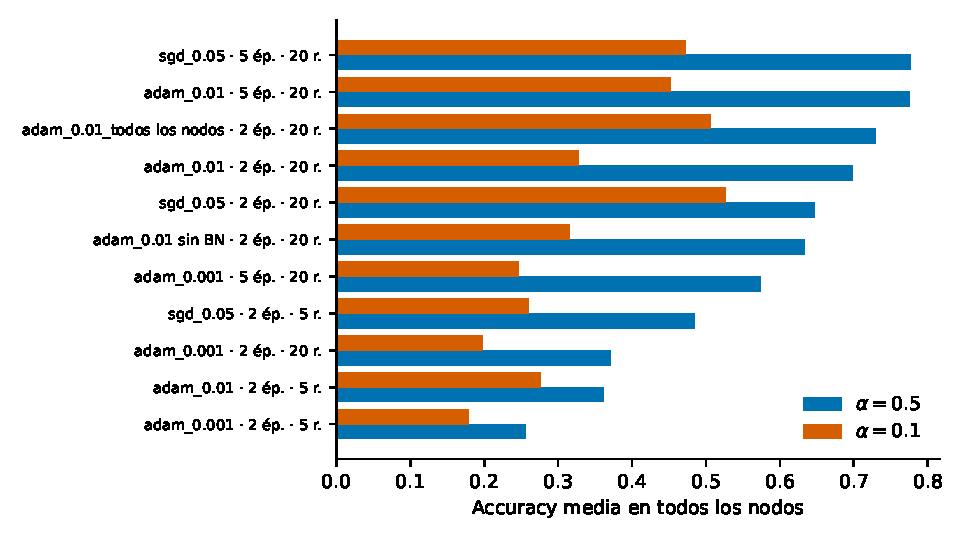
\includegraphics[width=0.78\linewidth]{fig_training.pdf}
\caption{Accuracy media en todos los nodos de una arquitectura fija según la configuración de FedAvg ($C=10$ nodos aleatorios, salvo ``todos los nodos''). Una sola partición.}\label{fig:training}\end{figure}

\subsection{Calidad del estimador de fitness}
\begin{figure}[H]\centering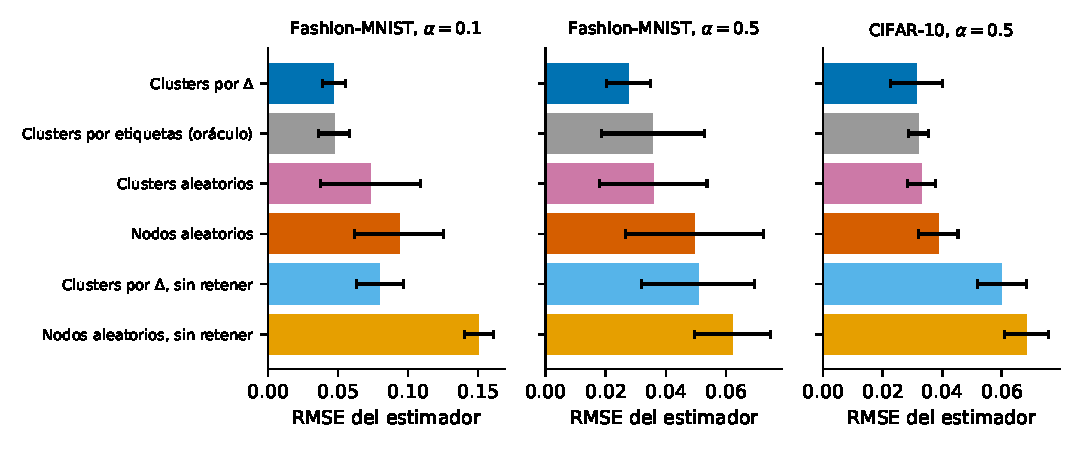
\includegraphics[width=\linewidth]{fig_e2.pdf}
\caption{RMSE del estimador por variante y régimen (media $\pm$ DE entre semillas; $C=10$). Fashion-MNIST con Adam $10^{-2}$ y 20 rondas (5 semillas por $\alpha$); CIFAR-10 con Adam $10^{-3}$ y 8 rondas (5 semillas), donde los modelos casi no aprenden (accuracy $\approx$0.21).}\label{fig:e2}\end{figure}
\begin{table}[H]\centering\small\caption{Estimador de fitness frente a la accuracy del mismo modelo en todos los nodos (media sobre semillas; DE = desviación entre semillas; $\tau$: Kendall dentro de cada sorteo).}\label{tab:e2}
\resizebox{\linewidth}{!}{%
\begin{tabular}{llrrrrr}
\toprule
Régimen & Variante & Sesgo & RMSE & RMSE (DE) & $\tau$ & Semillas \\
\midrule
Fashion-MNIST, $\alpha=0.1$ & Clusters por $\Delta$ & -0.008 & 0.047 & 0.008 & 0.885 & 5 \\
Fashion-MNIST, $\alpha=0.1$ & Clusters por etiquetas (oráculo) & -0.012 & 0.047 & 0.011 & 0.900 & 5 \\
Fashion-MNIST, $\alpha=0.1$ & Clusters aleatorios & -0.001 & 0.073 & 0.036 & 0.886 & 5 \\
Fashion-MNIST, $\alpha=0.1$ & Nodos aleatorios & -0.036 & 0.094 & 0.032 & 0.853 & 5 \\
Fashion-MNIST, $\alpha=0.1$ & Clusters por $\Delta$, sin retener & 0.072 & 0.080 & 0.017 & 0.907 & 5 \\
Fashion-MNIST, $\alpha=0.1$ & Nodos aleatorios, sin retener & 0.140 & 0.151 & 0.010 & 0.868 & 5 \\
Fashion-MNIST, $\alpha=0.5$ & Clusters por $\Delta$ & 0.007 & 0.028 & 0.007 & 0.958 & 5 \\
Fashion-MNIST, $\alpha=0.5$ & Clusters por etiquetas (oráculo) & 0.003 & 0.036 & 0.017 & 0.957 & 5 \\
Fashion-MNIST, $\alpha=0.5$ & Clusters aleatorios & -0.004 & 0.036 & 0.018 & 0.952 & 5 \\
Fashion-MNIST, $\alpha=0.5$ & Nodos aleatorios & -0.015 & 0.049 & 0.023 & 0.945 & 5 \\
Fashion-MNIST, $\alpha=0.5$ & Clusters por $\Delta$, sin retener & 0.044 & 0.051 & 0.019 & 0.948 & 5 \\
Fashion-MNIST, $\alpha=0.5$ & Nodos aleatorios, sin retener & 0.053 & 0.062 & 0.013 & 0.972 & 5 \\
CIFAR-10, $\alpha=0.5$ & Clusters por $\Delta$ & 0.003 & 0.031 & 0.009 & 0.835 & 5 \\
CIFAR-10, $\alpha=0.5$ & Clusters por etiquetas (oráculo) & -0.002 & 0.032 & 0.003 & 0.829 & 5 \\
CIFAR-10, $\alpha=0.5$ & Clusters aleatorios & -0.002 & 0.033 & 0.005 & 0.823 & 5 \\
CIFAR-10, $\alpha=0.5$ & Nodos aleatorios & -0.015 & 0.039 & 0.007 & 0.819 & 5 \\
CIFAR-10, $\alpha=0.5$ & Clusters por $\Delta$, sin retener & 0.056 & 0.060 & 0.008 & 0.867 & 5 \\
CIFAR-10, $\alpha=0.5$ & Nodos aleatorios, sin retener & 0.062 & 0.068 & 0.007 & 0.850 & 5 \\
\bottomrule
\end{tabular}}
\end{table}

Tres hechos se sostienen. (1) El evaluador retenido reduce el RMSE un 41--48\,\% con clusters por $\Delta$ (21--43\,\% con nodos aleatorios) y lleva el sesgo de $+0.04$--$+0.14$ a valores entre $-0.04$ y $+0.01$ en los tres regímenes. (2) Los clusters por $\Delta$ capturan estructura de etiquetas sin verlas: la fracción de varianza de la distribución de clases que explican es 0.71 con $\alpha=0.1$ (0.80 el oráculo con etiquetas, 0.10 el azar) y 0.48 con $\alpha=0.5$ (0.62 el oráculo); con $\alpha=0.1$ igualan al oráculo en RMSE. (3) Frente a muestrear nodos al azar, el RMSE de los clusters por $\Delta$ es menor en Fashion-MNIST ($+0.047$ de diferencia pareada con IC $[0.024,0.076]$ para $\alpha=0.1$, mejor en 5/5 semillas; $+0.022$ $[0.003,0.041]$ para $\alpha=0.5$) y no se detecta diferencia en CIFAR-10 con modelos sin entrenar. Pero el \emph{ranking} no mejora: $\tau$ va de 0.82 a 0.97 en todas las variantes y regímenes, sin diferencias claras entre ellas. Por tanto el estimador es más exacto, no más ordenador.

\subsection{Búsqueda de frentes (E3)}
Fashion-MNIST, $\alpha=0.1$, $N=100$, $C=10$, población 10, 8 generaciones (150 evaluaciones, 30\,000 entrenamientos locales de búsqueda por corrida y método, idénticos). Cuatro métodos con la misma partición, sonda y semilla (la búsqueda aleatoria con clusters y la búsqueda aleatoria con nodos aleatorios evalúan exactamente las mismas 150 arquitecturas por semilla; los dos NSGA-II comparten su población inicial, que difiere de la de las búsquedas aleatorias, lo que explica que su HV en la generación 0 difiera): CS-NSGA (la propuesta), NSGA-II con 10 nodos al azar por generación, búsqueda aleatoria con los mismos clusters y, como control, búsqueda aleatoria con nodos aleatorios.
\begin{figure}[H]\centering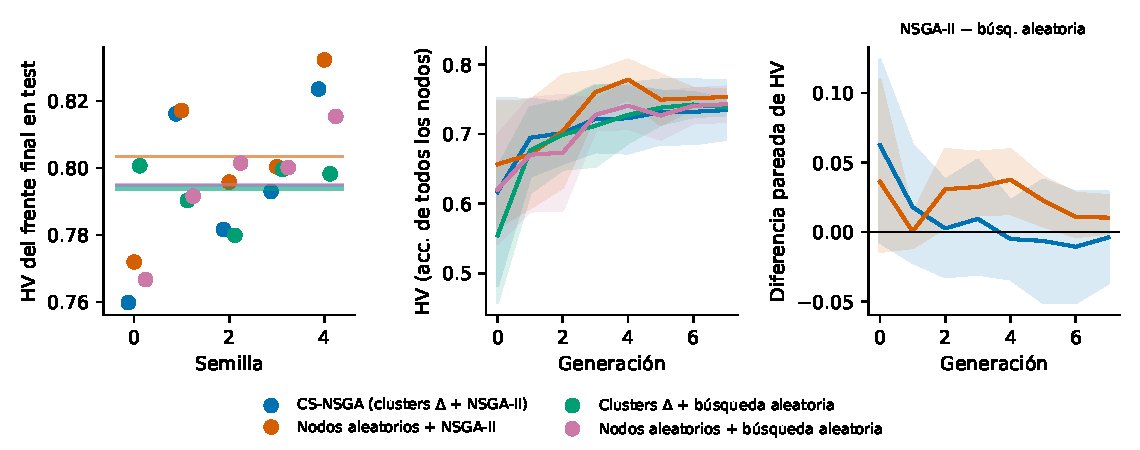
\includegraphics[width=\linewidth]{fig_e3.pdf}
\caption{Izquierda: HV del frente final en test por semilla (líneas: medias). Centro: HV del archivo con la accuracy de todos los nodos por generación (media $\pm$ DE). Derecha: diferencia pareada por semilla de ese HV entre NSGA-II y la búsqueda aleatoria con el mismo muestreo de nodos (azul: clusters; naranja: nodos aleatorios), por generación (banda: IC bootstrap al 95\,\% sobre 5 semillas; 0 = sin diferencia). La búsqueda aleatoria parte de otra población inicial, por lo que las diferencias de las primeras generaciones reflejan en parte el azar de esa población.}\label{fig:e3}\end{figure}
\begin{table}[H]\centering\small\caption{E3: frente final reevaluado en test (media $\pm$ DE, 5 semillas) y calidad del estimador durante la búsqueda.}\label{tab:e3}
\resizebox{\linewidth}{!}{%
\begin{tabular}{lllrrr}
\toprule
Método & HV test & HV todos los nodos & RMSE est. & $\tau$ est. & Entren. locales \\
\midrule
CS-NSGA (clusters $\Delta$ + NSGA-II) & 0.795 $\pm$ 0.026 & 0.735 & 0.043 & 0.908 & 30000 \\
Clusters $\Delta$ + búsqueda aleatoria & 0.794 $\pm$ 0.009 & 0.738 & 0.045 & 0.893 & 30000 \\
Nodos aleatorios + NSGA-II & 0.804 $\pm$ 0.023 & 0.753 & 0.077 & 0.883 & 30000 \\
Nodos aleatorios + búsqueda aleatoria & 0.795 $\pm$ 0.018 & 0.743 & 0.077 & 0.867 & 30000 \\
\bottomrule
\end{tabular}}
\end{table}

\begin{table}[H]\centering\small\caption{E3: diferencias pareadas por semilla (IC bootstrap sobre 5 semillas; descriptivo).}\label{tab:e3c}
\resizebox{\linewidth}{!}{%
\begin{tabular}{llrrr}
\toprule
Contraste & Métrica & Diferencia & IC 95 \% & A favor \\
\midrule
CS-NSGA $-$ NSGA-II nodos aleat. & HV test & -0.009 & [-0.012, -0.005] & 0/5 \\
CS-NSGA $-$ NSGA-II nodos aleat. & HV todos (final) & -0.019 & [-0.055, 0.017] & 3/5 \\
CS-NSGA $-$ NSGA-II nodos aleat. & Área bajo la curva & -0.021 & [-0.060, 0.018] & 2/5 \\
NSGA-II nodos aleat. $-$ búsq. aleat. nodos aleat. & HV test & 0.008 & [-0.001, 0.019] & 4/5 \\
NSGA-II nodos aleat. $-$ búsq. aleat. nodos aleat. & HV todos (final) & 0.010 & [-0.001, 0.027] & 4/5 \\
NSGA-II nodos aleat. $-$ búsq. aleat. nodos aleat. & Área bajo la curva & 0.023 & [0.016, 0.029] & 5/5 \\
CS-NSGA $-$ búsq. aleat. clusters & HV test & 0.001 & [-0.021, 0.021] & 3/5 \\
CS-NSGA $-$ búsq. aleat. clusters & HV todos (final) & -0.004 & [-0.037, 0.029] & 3/5 \\
CS-NSGA $-$ búsq. aleat. clusters & Área bajo la curva & 0.008 & [-0.027, 0.038] & 3/5 \\
búsq. aleat. clusters $-$ búsq. aleat. nodos aleat. & HV test & -0.001 & [-0.017, 0.017] & 1/5 \\
búsq. aleat. clusters $-$ búsq. aleat. nodos aleat. & HV todos (final) & -0.004 & [-0.022, 0.013] & 1/5 \\
búsq. aleat. clusters $-$ búsq. aleat. nodos aleat. & Área bajo la curva & -0.007 & [-0.018, 0.005] & 1/5 \\
NSGA-II nodos aleat. $-$ búsq. aleat. clusters & HV test & 0.010 & [-0.011, 0.028] & 4/5 \\
NSGA-II nodos aleat. $-$ búsq. aleat. clusters & HV todos (final) & 0.015 & [0.009, 0.023] & 5/5 \\
NSGA-II nodos aleat. $-$ búsq. aleat. clusters & Área bajo la curva & 0.029 & [0.013, 0.045] & 4/5 \\
\bottomrule
\end{tabular}}
\end{table}

La propuesta no mejora el frente. Frente a NSGA-II con nodos aleatorios es ligeramente peor, y de forma consistente (la desviación pareada es de solo 0.005): $-0.009$ de HV ($\approx$1\,\%) con 0 de 5 semillas a favor. \textbf{Sí hay evolución en las curvas, y su atribución depende del muestreo.} El HV del archivo con la accuracy de todos los nodos sube de la generación 0 a la 7 en los cuatro métodos (Figura~\ref{fig:e3}, centro): $+0.118$ con CS-NSGA (mejora en 4/5 semillas), $+0.097$ con NSGA-II y nodos aleatorios (5/5), $+0.184$ con la búsqueda aleatoria con clusters y $+0.122$ con la búsqueda aleatoria con nodos aleatorios (5/5 ambas), que parten de poblaciones iniciales distintas. Con los mismos clusters, la diferencia pareada entre NSGA-II y búsqueda aleatoria es compatible con cero en todas las generaciones (de $+0.018$ en la generación 1 a $-0.004$ en la 7; Figura~\ref{fig:e3}, derecha, azul) y en el área bajo la curva ($+0.008$, $[-0.027,+0.038]$). Con nodos aleatorios, en cambio, NSGA-II queda por encima de la búsqueda aleatoria en el área bajo la curva en las 5 semillas ($+0.023$, $[+0.016,+0.029]$; Figura~\ref{fig:e3}, derecha, naranja) y por poco en el HV final (test $+0.008$, $[-0.001,+0.019]$, 4/5; todos los nodos $+0.010$, $[-0.001,+0.027]$, 4/5): un efecto pequeño (hasta $\approx$3\,\% del HV medio) pero consistente. Que el muestreo por clusters no tenga búsqueda aleatoria distinta del muestreo aleatorio ($-0.001$, $[-0.017,+0.017]$) sugiere que la diferencia aparece en la combinación con NSGA-II; una explicación coherente con el estudio de ruido, no probada, es que a $C=10$ los clusters dan modelos más ruidosos y sesgados que los nodos aleatorios, lo que degrada la selección. El HV por generación se calcula sobre el frente que elige cada algoritmo con su estimación ruidosa, por lo que no es monótono. La diferencia mínima detectable de este diseño para un contraste con una desviación pareada como la de CS-NSGA frente a la búsqueda con clusters es de $\approx0.046$ (5.7\,\% del HV con 80\,\% de potencia), de modo que efectos menores no se habrían visto en ese contraste. Conviene además no usar el HV calculado con la accuracy estimada por los representantes: favorece a los nodos aleatorios (0.837 frente a 0.771) y esa ventaja desaparece con la accuracy de todos los nodos y con test, un caso de optimismo por selección sobre un estimador más ruidoso.

\subsection{Por qué: paisaje con estructura y fitness ruidoso}
\textbf{El paisaje no es plano.} Entre 150 arquitecturas aleatorias por semilla la accuracy media es 0.38 con desviación 0.157 y rango 0.06--0.76; solo el 1\,\% está a $\le0.02$ de la mejor y el 3\,\% a $\le0.05$. Los genes explican el 65\,\% de la varianza (validación cruzada de un bosque aleatorio), sobre todo el número de bloques y el dropout. Hay, pues, estructura que una búsqueda dirigida podría explotar.

\textbf{El ruido del fitness es del tamaño de la banda de las mejores.} Entrenar la misma arquitectura con otros 10 nodos cambia su accuracy global en $\pm0.058$ (a partir de las reevaluaciones del propio E3) frente a 0.18 de desviación entre arquitecturas, igual con clusters que con nodos aleatorios. Un estudio específico (20 arquitecturas aleatorias, 4 sorteos de los nodos de entrenamiento, una partición) lo cuantifica por número de nodos (Figura~\ref{fig:noise}, Tabla~\ref{tab:noise}).
\begin{figure}[H]\centering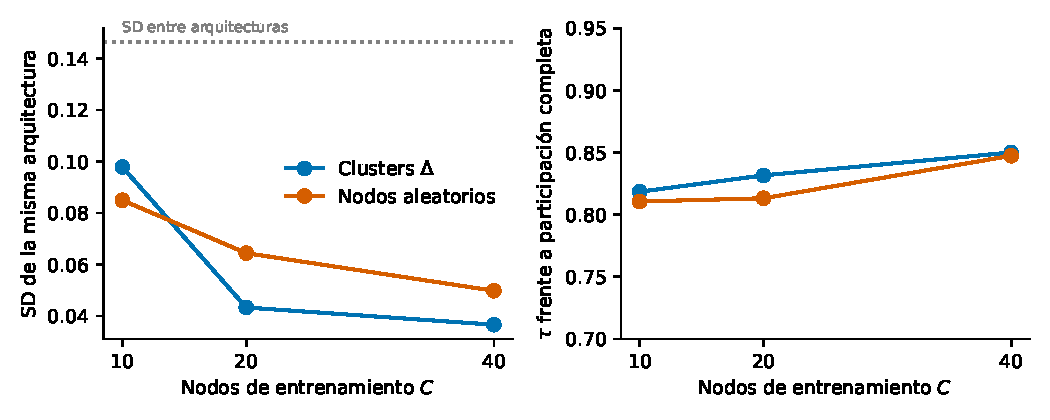
\includegraphics[width=0.92\linewidth]{fig_noise.pdf}
\caption{Izquierda: desviación de la accuracy de una misma arquitectura al cambiar los nodos de entrenamiento. Derecha: Kendall $\tau$ frente a la accuracy con participación completa (un sorteo).}\label{fig:noise}\end{figure}
\begin{table}[H]\centering\small\caption{Ruido por nodos de entrenamiento (20 arquitecturas $\times$ 4 sorteos, Fashion-MNIST, $\alpha=0.1$).}\label{tab:noise}
\resizebox{\linewidth}{!}{%
\begin{tabular}{lrrrrrr}
\toprule
Variante & SD misma arq. & Ruido/señal & $\tau$ test-retest & $\tau$ vs completa & Sesgo vs completa & RMSE vs completa \\
\midrule
Clusters $\Delta$, $C=10$ & 0.098 & 0.695 & 0.746 & 0.818 & -0.166 & 0.195 \\
Clusters $\Delta$, $C=20$ & 0.043 & 0.283 & 0.796 & 0.832 & -0.083 & 0.101 \\
Clusters $\Delta$, $C=40$ & 0.037 & 0.243 & 0.830 & 0.850 & -0.067 & 0.082 \\
Nodos aleatorios, $C=10$ & 0.085 & 0.650 & 0.747 & 0.811 & -0.113 & 0.145 \\
Nodos aleatorios, $C=20$ & 0.064 & 0.442 & 0.819 & 0.813 & -0.064 & 0.095 \\
Nodos aleatorios, $C=40$ & 0.050 & 0.321 & 0.825 & 0.847 & -0.026 & 0.063 \\
\bottomrule
\end{tabular}}
\end{table}

Con $C=10$ el ruido es el más alto (relación ruido/señal $\approx$0.65--0.70 en esta muestra; $\approx$0.32 con los datos de E3, discrepancia no reconciliada por tratarse de conjuntos de arquitecturas distintos). Pasar a $C=20$ lo reduce a menos de la mitad con clusters (0.098$\to$0.043) y mucho menos con nodos aleatorios (0.085$\to$0.064); de 20 a 40 apenas cambia. Agrupar por $\Delta$ reduce el ruido solo con $C\ge20$. Sin embargo, el orden frente a participación completa casi no mejora con $C$ ($\tau\approx0.81$--$0.85$) y, entre arquitecturas separadas por menos de 0.05, se acierta el orden en solo el 61--72\,\% de los pares sin tendencia clara con $C$ ni con el método. Entrenar con pocos nodos además subestima la accuracy (entre $-0.03$ y $-0.17$). Todo ello encaja con el resultado de E3: a $C=10$ los clusters no reducen el ruido de entrenamiento y se alejan más de la accuracy completa que los nodos aleatorios; su ventaja es de \emph{evaluación}, no de entrenamiento. Es una explicación coherente, no una prueba: E3 con $C=20$ no se ha ejecutado.

\subsection{Refinamiento multifidelidad (E4)}
Sobre las 20 corridas de E3 (incluido el control) se reevaluaron los $\le12$ candidatos más prometedores con $C=40$ nodos aleatorios nuevos (coste añadido de $\approx$9\,600 entrenamientos locales por corrida, el mismo para los cuatro métodos), se eligió el frente final con esa estimación y se reentrenó con participación completa.
\begin{table}[H]\centering\small\caption{E4: HV del frente final en test antes y después del refinamiento multifidelidad ($C=40$ sobre $\leq 12$ candidatos).}\label{tab:e4}
\resizebox{\linewidth}{!}{%
\begin{tabular}{lrrrrr}
\toprule
Método & HV original & HV refinado & Cambio pareado & IC 95 \% & Mejoran \\
\midrule
CS-NSGA (clusters $\Delta$ + NSGA-II) & 0.795 & 0.794 & -0.001 & [-0.010, 0.004] & 4/5 \\
Clusters $\Delta$ + búsqueda aleatoria & 0.794 & 0.798 & 0.005 & [0.001, 0.009] & 5/5 \\
Nodos aleatorios + NSGA-II & 0.804 & 0.812 & 0.009 & [0.001, 0.017] & 4/5 \\
Nodos aleatorios + búsqueda aleatoria & 0.795 & 0.794 & -0.001 & [-0.026, 0.017] & 3/5 \\
\bottomrule
\end{tabular}}
\end{table}

El refinamiento aporta como mucho $+0.005$ a $+0.009$ de HV ($\approx$1\,\%) en dos de cuatro métodos (NSGA-II con nodos aleatorios y búsqueda aleatoria con clusters) y nada en CS-NSGA ni en la búsqueda aleatoria con nodos aleatorios ($-0.001$); no cambia el orden entre métodos (la diferencia CS-NSGA frente a NSGA con nodos aleatorios pasa a $-0.019$, $[-0.031,-0.006]$) y la mejor accuracy de test apenas se mueve ($-0.005$ a $+0.003$). La estimación refinada correlaciona 0.99 con la accuracy del mismo modelo en todos los nodos (0.92 la de búsqueda con $C=10$), pero eso no se traduce en mejores frentes con entrenamiento completo: el cuello de botella parece estar en el conjunto de candidatos que genera la búsqueda y en la diferencia entre entrenar con $C$ nodos y con todos.

\section{Discusión}
\textbf{Qué se sostiene.} Evaluar en un nodo retenido del cluster es un cambio sencillo y reproducido en cuatro estudios que reduce el sesgo y el error de un estimador de fitness basado en pocos nodos; los clusters por actualizaciones aproximan a los de etiquetas sin revelar etiquetas, algo que, según nuestra lectura, los grupos balanceados por distribución de etiquetas de \cite{yuan2022resourceaware} no ofrecen. \textbf{El mejor método en promedio es el más simple.} NSGA-II con nodos aleatorios obtiene el mayor HV en test (0.804 frente a 0.795, 0.794 y 0.795), con el HV de todos los nodos (0.753 frente a 0.735, 0.739 y 0.743), tras el refinamiento (0.812) y en el área bajo la curva de HV. Su ventaja sobre CS-NSGA es pequeña ($\approx$1\,\%) pero consistente (0 de 5 semillas a favor de CS-NSGA). Frente a la búsqueda aleatoria con el mismo muestreo (el control que cierra la confusión anterior) la ventaja es pequeña y consistente en el área bajo la curva (5/5) y sugerente en el HV final. La parte de clusters de la propuesta no ayuda a la búsqueda en este régimen, y la evolución parece aportar algo solo cuando el muestreo es aleatorio. \textbf{Qué no.} Esa mejora de la evaluación no se tradujo en mejores frentes: a $C=10$ el limitante es el ruido del fitness por \emph{qué nodos entrenan}, que ni la estratificación ni el refinamiento posterior corrigen, y que impide ordenar bien a las mejores arquitecturas con una sola evaluación. Es coherente con la advertencia de \cite{khodak2021federated} sobre la validación ruidosa con pocos clientes, que aquí se cuantifica y se descompone entre evaluación y entrenamiento. \textbf{Relación con la literatura.} En espacios mucho mayores la búsqueda aleatoria sí pierde frente a una dirigida a igual presupuesto \cite{dudziak2022fedoras}; nuestro espacio es pequeño y el presupuesto bajo, lo que puede explicar que el efecto de NSGA-II sea pequeño, pero este informe no lo prueba.

\section{Limitaciones y amenazas a la validez}
\begin{itemize}[leftmargin=*,itemsep=1pt]
\item Cinco semillas por contraste; los intervalos bootstrap sobre cinco valores son descriptivos. La evolución no podría haberse detectado por debajo de $\approx$5.7\,\% de HV.
\item El frente final se reevalúa con una sola semilla de inicialización y como máximo 5 arquitecturas por frente; E3 y E4 usan un solo conjunto de datos, un solo $\alpha$ (0.1) y $C=10$.
\item Los estudios de estimador y ruido usan arquitecturas aleatorias, no las que genera una búsqueda; el estudio de ruido usa una sola partición y 20 arquitecturas, y sus desviaciones y $\tau$ son estimaciones ruidosas sin intervalos.
\item Espacio de búsqueda pequeño; presupuesto de 150 evaluaciones; no se ablacionó la ponderación por tamaño de cluster ni el método de agrupamiento.
\item El refinamiento ocurre tras la búsqueda y no la guía; no se probó el fitness acumulado entre generaciones ni \emph{successive halving} dentro de la búsqueda.
\item Se corrigió a tiempo un error propio en el script de análisis del estudio de ruido (alineación de arquitecturas en el cálculo de $\tau$); las cifras presentadas son las corregidas.
\end{itemize}

\section{Conclusiones y trabajo futuro}
CS-NAS, tal como se implementó y con el régimen y presupuesto probados, no mejora la búsqueda de arquitecturas frente a muestrear nodos al azar (es ligeramente peor que NSGA-II con nodos aleatorios) y la evolución no se distingue de la búsqueda aleatoria cuando se usan clusters. Con muestreo aleatorio de nodos, NSGA-II supera a la búsqueda aleatoria por un margen pequeño pero consistente en el área bajo la curva de HV (5/5 semillas) y sugerente en el HV final. El método con mejores cifras es, por tanto, NSGA-II con nodos aleatorios. El resultado útil es de diagnóstico: el evaluador retenido, un estimador por clusters de $\Delta$ más exacto que el aleatorio, y la caracterización del ruido de fitness por nodos de entrenamiento como cuello de botella. Los siguientes pasos de mayor valor informativo son: (1) repetir E3 con $C=20$ y más semillas, la única prueba directa de que el ruido era el obstáculo (el doble de coste); (2) fitness multifidelidad \emph{dentro} de la búsqueda (acumular evaluaciones de los padres, descarte temprano); (3) un espacio de búsqueda mayor o un segundo conjunto de datos, donde la evolución tendría más margen.

\section{Reproducibilidad}
Rama \texttt{experiment/cluster-sampling-nas}; el código de las propuestas anteriores está en la etiqueta \texttt{legacy-final} y sus resultados en \texttt{\~{}/Desktop/evofederated\_legacy\_results.tar.gz}. Los resultados de este informe están en \texttt{runs/} (no versionado; copia en \texttt{\~{}/Desktop/evofederated\_cs\_nas\_runs.tar.gz}) y las decisiones y resultados detallados en \texttt{docs/} (\texttt{PROTOCOL}, \texttt{E3\_DESIGN}, \texttt{E4\_DESIGN}, \texttt{RESULTS\_*}, \texttt{ANALISIS\_CONSOLIDADO}). Código: \texttt{run\_cs.py} (una corrida), \texttt{run\_estimator\_study.py}, \texttt{run\_training\_diagnostic.py}, \texttt{run\_noise\_study.py}, \texttt{run\_refine.py} y los \texttt{analyze\_*.py}; las figuras y tablas de este informe se generan con \texttt{manuscript/make\_report\_assets.py} a partir de \texttt{runs/}. Las semillas de cada corrida se guardan en su \texttt{config.json}. El estado del código aún no está confirmado en git (cambios sin commit en el momento de redactar).

\bibliographystyle{unsrt}
\bibliography{references_included,background}
\end{document}
